\documentclass[a4paper,12pt]{article}
\usepackage[english]{babel}
\usepackage[latin1]{inputenc}
\usepackage{amsmath}
\usepackage{amssymb}
\usepackage{amsfonts}
\usepackage{graphicx}
\usepackage{listings}
\usepackage{xcolor}
\usepackage{color}

\usepackage[colorinlistoftodos]{todonotes}
\usepackage[toc,page]{appendix}
\usepackage{geometry}
 \geometry{
 a4paper,
 total={170mm,257mm},
 left=20mm,
 top=20mm,
 }
 \usepackage{hyperref}
 \hypersetup{
    bookmarks=true,         % show bookmarks bar?
    unicode=false,          % non-Latin characters in Acrobat’s bookmarks
    pdftoolbar=true,        % show Acrobat’s toolbar?
    pdfmenubar=true,        % show Acrobat’s menu?
    pdffitwindow=false,     % window fit to page when opened
    pdfstartview={FitH},    % fits the width of the page to the window
    pdftitle={My title},    % title
    pdfauthor={Author},     % author
    pdfsubject={Subject},   % subject of the document
    pdfcreator={Creator},   % creator of the document
    pdfproducer={Producer}, % producer of the document
    pdfkeywords={keyword1, key2, key3}, % list of keywords
    pdfnewwindow=true,      % links in new PDF window
    colorlinks=false,       % false: boxed links; true: colored links
    linkcolor=red,          % color of internal links (change box color with linkbordercolor)
    citecolor=green,        % color of links to bibliography
    filecolor=magenta,      % color of file links
    urlcolor=cyan           % color of external links
}

\begin{document}
\begin{titlepage}
%----------------------------------------------------------------------------------------
%	HEADING SECTIONS
%----------------------------------------------------------------------------------------
\newcommand{\HRule}{\rule{\linewidth}{0.5mm}} % Defines a new command for the horizontal lines, change thickness here
\setlength{\topmargin}{0in}
\center % Center everything on the page
 
 \begin{minipage}{0.4\textwidth}
\begin{flushleft} \large
\hspace*{-0.5cm}

\includegraphics[scale=4]{images/uni_logo.png}\\
\end{flushleft}
\end{minipage}
~
\begin{minipage}{0.5\textwidth}
\begin{flushright} \large
\hspace*{2cm}

\includegraphics[scale=0.6]{images/fac_logo.png}\\
\end{flushright}
\end{minipage}\\[1cm]

\textsc{\Large Cairo University - Faculty of Engineering}\\[0.5cm] % Major
\textsc{Computer Engineering Department} \\[0.5cm] 
\textsc{Marketing - Spring 2020} \\[0.5cm] 
% Name of your heading such as course name
\textsc{\large }\\[0.5cm] % Minor heading such as course title

%----------------------------------------------------------------------------------------
%	TITLE SECTION
%----------------------------------------------------------------------------------------

\HRule \\[0.4cm]
{ \huge \bfseries Google Stadia}\\[0.4cm] % Title of your document
\HRule \\[1cm]
 
%----------------------------------------------------------------------------------------
%	AUTHOR SECTION
%----------------------------------------------------------------------------------------
\begin{minipage}{0.8\textwidth}
\begin{flushleft} 
\textbf{Mohamed Shawky Zaky} \\
\texttt{SEC:1, BN:20} \\[0.5cm]

\textbf{Remonda Talaat Eskarous} \\
\texttt{SEC:1, BN:20} \\[0.5cm]

\textbf{Evram Youssef Helmy} \\
\texttt{SEC:1, BN:9} \\[0.5cm]

\textbf{Mahmoud Osman Adas} \\
\texttt{SEC:2, BN:21} \\[0.5cm]

\textbf{Kareem Omar Mostafa} \\
\texttt{SEC:2, BN:6} \\[0.5cm]
\end{flushleft}
\end{minipage}\\[6cm]

\end{titlepage}

\thispagestyle{empty}

\tableofcontents
\listoffigures
\clearpage

\pagenumbering{arabic}

%----------------------------------------------------------------------------------------
%	REPORT SECTIONS
%----------------------------------------------------------------------------------------
\section{Introduction}
Stadia is a new gaming platform by Google which is presented as the next evolution
of console gaming. The video gaming industry as it stands consists of several 
integral parts (as of now) one of which is the gaming console (Fig. \ref{fig:consoles}). The gaming 
console is the hardware necessary to experience video games. It can be expensive, 
hard to maintain and become irrelevant after several years of use (which requires 
purchasing a new console with new hardware).

\begin{figure}[H]
    \centering
    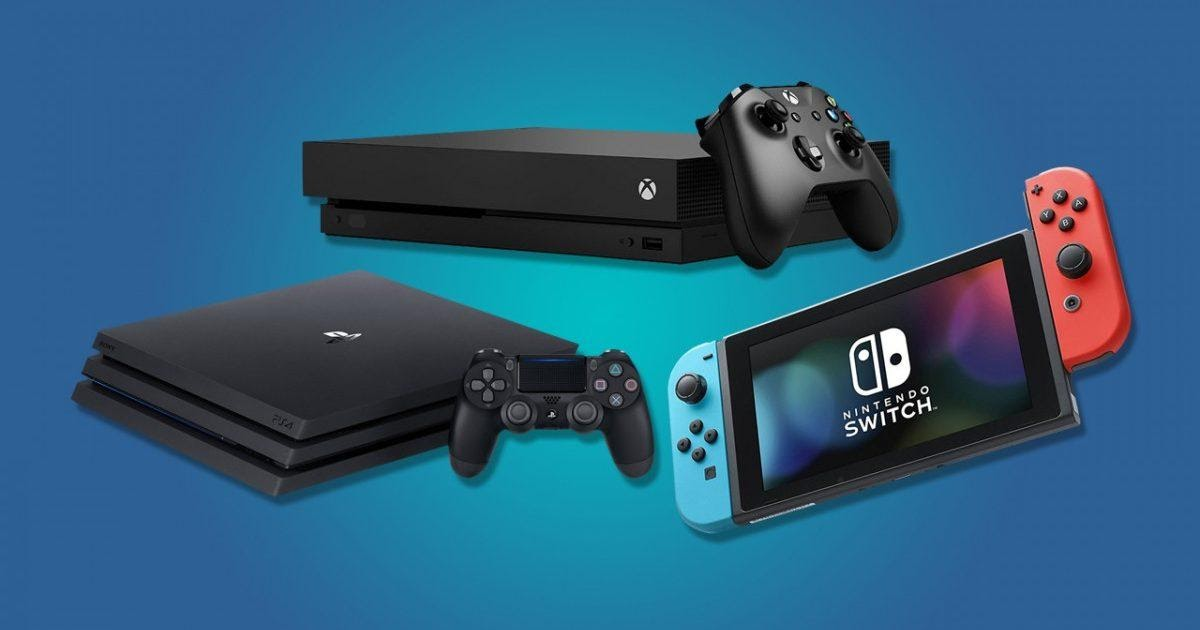
\includegraphics[width=10cm]{images/consoles.jpg}
    \caption{Gaming Consoles}
    \label{fig:consoles}
\end{figure}

Stadia tries to eliminate the console by offering video gaming as a subscription 
service like streaming services (Hulu, Netflix, etc...). with internet speed on the rise 
with the cloud computing industry taking shape, the possibility of removing the 
need of specialized hardware for gaming is increasing.
In this paper, we take a closer look on Stadia, what it does right, what is does wrong
and what can it do to achieve its goals.


\section{Type of Product}
Stadia can be classified as an augmented service as the main purchasable is a subscription-based service that can't be access without a sufficiently high internet speed connection (a minimum of 10Mbps according to their website \cite{stadiaSupport}) so it can't 
be a product as a product must be tangible and can be consumed at will without a special requirement(internet connection).

\begin{figure}[H]
    \centering
    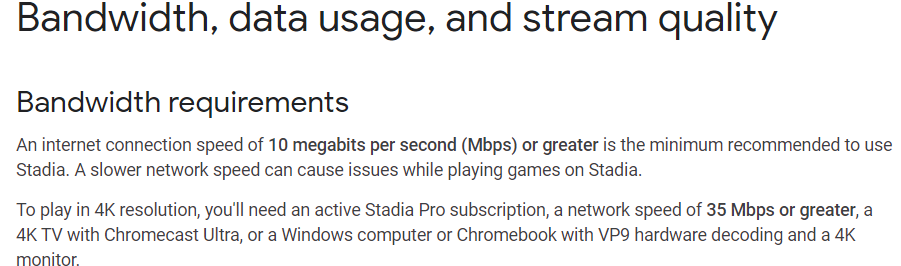
\includegraphics[width=13cm]{images/bandwidth.png}
    \caption{Screen Capture Of Internet Requirement}
    \label{fig:internetReq}
\end{figure}

As for the augmented part, Stadia subscriptions include (optional) products to use 
with the service such as the Stadia controller.

\begin{figure}[H]
    \centering
    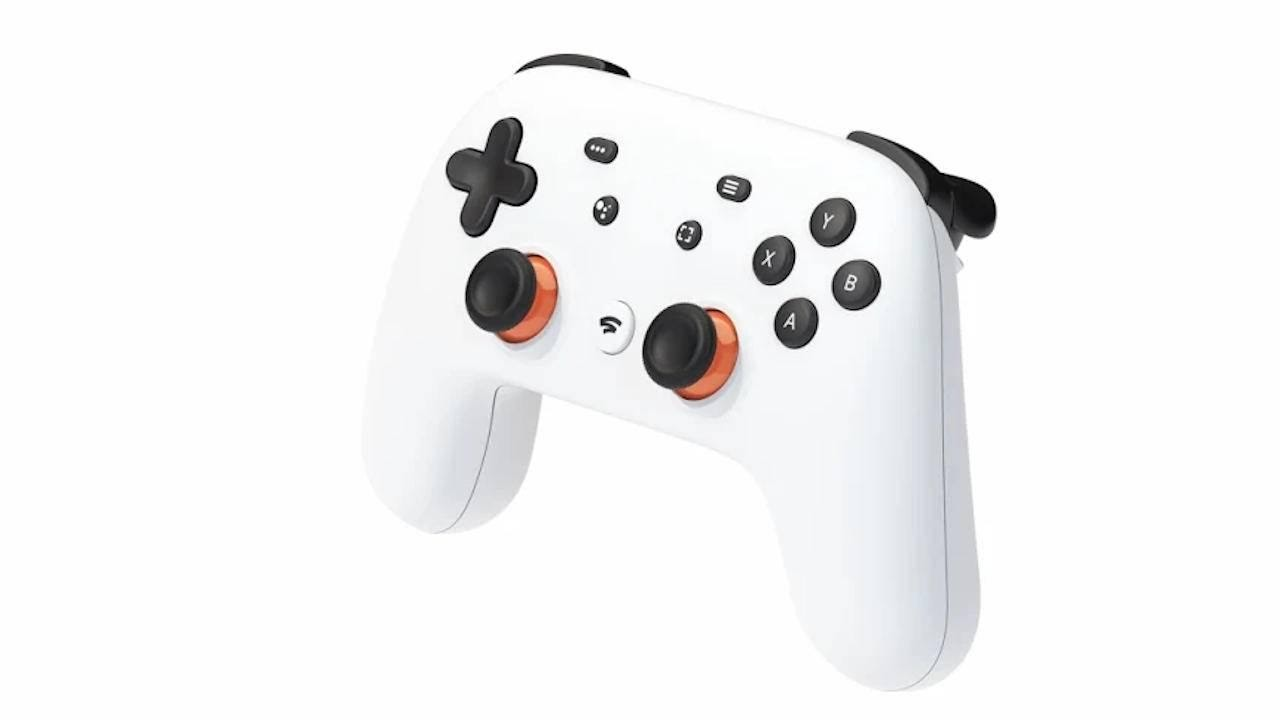
\includegraphics[width=10cm]{images/controller.jpg}
    \caption{Google Stadia Controller}
    \label{fig:controller}
\end{figure}

In conclusion, google Stadia is a service with optional products to enhance the 
experience.


\section{Marketing Mix}
In this section, we will discuss the \texttt{4P's Marketing Mix} of our research product \emph{(Google Stadia)}. We will discuss the product definition, its price analysis, its place and promotion. This helps us further understand the marketing setup of this new product and develop a common understand of how it begins and whether it will stand and succeed.

\begin{figure}[h]
    \centering
    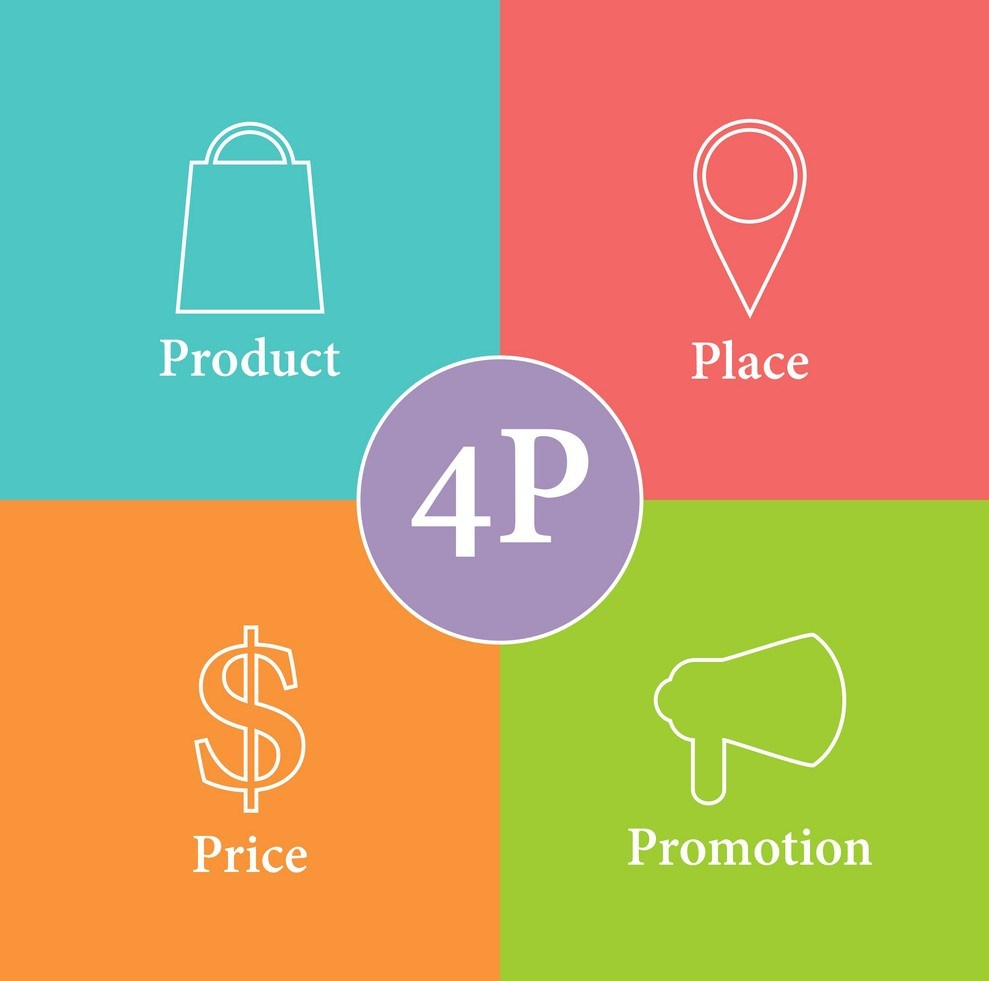
\includegraphics[width=0.5\textwidth]{images/4p.jpg}
    \caption{4P's Marketing Mix Diagram}
    \label{fig:4p}
\end{figure}

\subsection{Product}
As mentioned before, \emph{Google Stadia} is a cloud streaming service for video games, where gamers can stream video games, running on cloud systems, without having to buy the game console themselves. Stadia offers a very cheap way of playing videos games for gamers, who can't afford buying a game console or an expensive gaming rig. \\

To use Stadia service, the user just need a device with \emph{Google Chrome} or any Stadia-supported application on his/her personal computer or mobile phone and a reliable internet connection, in addition to the monthly subscription. \\

Stadia is not the first project of its kind. We have \emph{Nvidia Geforce Now} and \emph{Microsoft Project XCloud}. However, Stadia offers seamless $4K$ video game streaming based on \emph{Youtube} streaming service, which is a big bonus over other streaming services. 

\subsection{Price}
Stadia is subscription-based service, where the users pay a monthly fee, in order to use the service. There are two levels of membership: \emph{Stadia Pro}, which is paid for, and \emph{plain Stadia}, a free access plan. \\

\emph{Stadia Pro} offers the user a seamless $HDR$ $4K$ gaming experience, with a good library of video games. However, the user still has to purchase most of the video games on top of it. Stadia Pro membership costs $8.99$ $GBP$ per month in the UK, $\$9.99$ $USD$ per month in the US. New subscribers can get a free one-month trial of Pro membership. \\

The alternative plan is \emph{plain Stadia} (a.k.a. Stadia Base). In this plan, users must purchase any required video game themselves. Also, the streaming quality is limited to $1080p$. This comes with an advantage that user doesn't have to pay any monthly fee.

\subsection{Place}
Since Stadia is an online cloud streaming platform, it's available worldwide. It's unavailable only in \emph{Hawaii} and \emph{Guam}. However, such service can be unpopular in countries, where internet connectivity is limited, such as African countries.

\subsection{Promotion}
\texttt{Google} follows an online promotion campaign, through advertisement on online platforms such as \emph{Youtube}. Most of the details of the platform development can be found at their developers website \cite{stadia_website}. Open source contribution to the project is also applicable.  \\

The service also provides a one-month free trial for Pro membership to encourage different users to use their platform. \texttt{Google} is also enhancing the service by including more video games and improving the streaming performance.

\section{SWOT Analysis}
\subsection{Introduction}

SWOT stands for Strengths, Weaknesses, Opportunities, and Threats, SWOT Analysis helps you define
what your business is better at and what it is lacking from.

By analysing and studying your business you will run into some questions like:
{
\renewcommand\labelitemi{}
\begin{itemize}
    \item what do you have?
    \item what do you miss?
    \item what is open for you?
    \item what may harm your business in the future?
\end{itemize}
}
all these questions can be answered by providing a suitable SWOT Analysis of your business.

\begin{figure}[h]
    \centering
    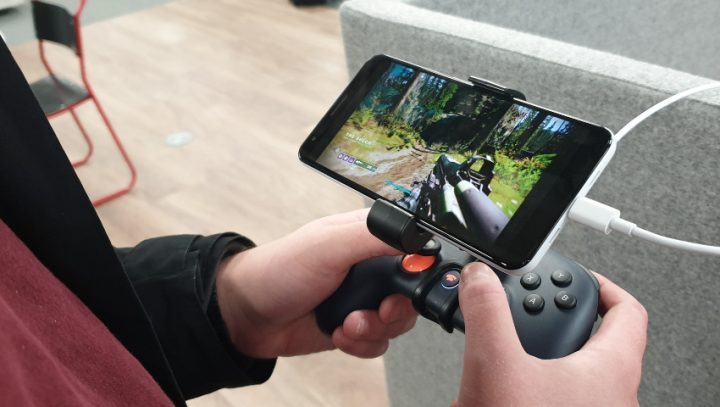
\includegraphics[width=0.8\textwidth]{images/stream.jpg}
    \caption{Stadia Game Stream}
    \label{fig:stream}
\end{figure}

\subsection{Strengths}
    \begin{itemize}
        \item \textbf{Gaming Experience:}
            Google Stadia offers a very well-established gaming stream for 
            their users, no delay or frame-drop, and the game controller is immediately reflected.
        \item \textbf{Google Image:}
            Google itself is the most clicked (visited) search-engine in the world
            this gives Stadia a great advantage since it's related to Google; on the contrary, companies
            like \emph{Tencent} and \emph{Walmart} will struggle more in marketing their competing product (service).
        \item \textbf{Content Creators:} 
            nowadays we have a large number of YouTubers (content creators), who stream their games and 
            upload it on their channels, since YouTube is one of Google's corporations Google Stadia
            easily offers full integration with YouTube for content, so no license are required, and 
            it becomes easily to upload your content.
    \end{itemize}

\subsection{Weaknesses}
\begin{itemize}    
    \item \textbf{Fiber:} 
        most of the world has turned their cables from TCP to Fiber however, some countries are still using
        old cable technologies, unfortunately Google Stadia requires the usage of Fiber cables,
        not only fast internet connection with $20mbs$, but also having Fiber cables.
    \item \textbf{Online Gaming:}
        even though Stadia offers a very good experience when playing, but sometimes the game controller
        may not be reflected, and the game may not respond, in offline games this is not a big issue, as you
        can respawn to your last checkpoint, but in online gaming this issue may but Stadia out of business.
    \item \textbf{Pricing:}
        as explained before, Stadia requires monthly fee and games are purchased separately, this demerit affect 
        gamers mostly, many people are purchasing gaming consoles (PS, XBOX) or even upgrading their PC for better gaming
        experience, and then purchase video games separately, so without a price plan for video games, Stadia is not
        offering them so much.
\end{itemize}

\subsection{Opportunities}
\begin{itemize}    
    \item \textbf{Unique:} 
        Google Stadia's strengths majorly lies in the uniqueness of their service,
        Cloud Gaming business is a brand new service not so many companies are competing in this
        area yet.

    \item \textbf{Leadership:}
        Stadia is the first of its kind, no major competitors yet, so they can add more features and obtain license for them
        before any other company does.
    
    \item \textbf{Gaming:}
        in total, there were an estimated 2.7 billion gamers across the globe in 2020, this creates a major opportunity
        for companies like Stadia.

    \item \textbf{Evolution:}
        as time goes by video games are evolving, and to have the best gaming experience you need to purchase the
        most recent gaming console, these consoles cost a lot, Stadia here appears to be a better solution
        for providing the same (sometimes better) gaming experience without the need of purchasing newer gaming
        consoles, so in order to achieve that they need to be always updated with the best technology.
\end{itemize}

\subsection{Threats}
\begin{itemize}    
    \item \textbf{Competitors:}
        the arising of other companies like Amazon and Microsoft, these major companies will have to compete against
        Stadia one day, and as huge as they are they will also come up with a huge marketing plan, and even better 
        promotion and pricing plans to overcome Stadia.

    \item \textbf{Gaming Consoles:}
        PS, XBOX and other companies can have similar   approach as google Stadia, allowing the user to play online 
        without the need of purchasing new gaming consoles, and overcome the problems google Stadia has regarding 
        online gaming.
\end{itemize}

\section{Pricing Strategy}
Stadia has 2 models:
\begin{enumerate}
    \item Stadia Pro.
    \item Stadia Base.
\end{enumerate}

\subsection{Stadia Pro}
Monthly subscription for \$9.99, let's you stream in 4K resolution and 5.1 surround sound.
Google selects you some games every now and then. \cite{stadiaPro}

Google priced `Stadia Pro' at \$9.99, which is a much lower price than its competitor Sony.
Sony - which owns `PlayStation Now' an old competitor for Stadia but only on PlayStation consoles - had its service priced at \$19.99. \cite{sonyPrices}

But after Google announced `Stadia Pro' pricing, Sony had to lower their prices to \$9.99.
Probably Google chose the `Penetration Pricing Strategy', and tried to draw attention from Sony's platform. \cite{pricingStategy}

\subsection{Stadia Base}
Free tier for the streaming, but you pay for the game which range between \$30 and \$60.
Not like Stadia Pro, with Stadia Base you will own the game.
Google caps the streaming quality of `Stadia Base' users to 1080p. \cite{stadiaBase}

Google is using `Stadia Base' as its `Fermium Pricing Strategy.'
It hopes that users will eventually pay to upgrade to `Stadia Pro' and use its full functionality.

With `Stadia Base', Google is also trying to fixing the issue of not owning the game - which a lot of people complained about.
Now you can own a game, Google will get revenue by acting as a store for those games, and can get customers for `Stadia Pro' using the fermium version.

\section{Promotion Strategy}
Before discussing the promotion strategy, let's define promotion types first.

\subsection{Promotion Types}
The Economist Times classifies \cite{promoTypes} promotion into:
\begin{enumerate}
    \item Press Releases.
    \item Advertising.
    \item Consumer Promotions.
    \item Trade Discounts.
    \item Freebies.
    \item Incentive Trips.
    \item Awards.
    \item Personal Selling.
\end{enumerate}
In the next subsections, we will discuss the different promotion techniques that google used with stadia.

\subsection{Press Release}
First and most notable way google promoted stadia was through their press release (conference) on March 2019 \cite{press}.

\begin{figure}[H]
    \centering
    
\includegraphics[width=10cm]{images/release.jpeg}
    \caption{Google CEO Sundar Pichai introduced Google's first major gaming initiative, Stadia, at the 2019 Game Developers Conference in March 2019. (Business Insider) \cite{businessInsiderCon}}
\end{figure}

\subsection{Advertising}
Google has a huge advantage in advertising compared to its competitors (Microsoft, Sony and Nintendo.)
Most of google's revenue comes from ads \cite{googleRevenue}. 

Google collects huge amounts of data to assist the advertisers in finding their target users. 
This data can help google a lot on choosing their target customers.
Google competitors don't have such huge amount of user data.

Nevertheless, Google didn't use that advantage very well. 
On its first trailer on Nov 19, 2019 \cite{stadiaTrailer}, stadia faced huge dislike from the gaming community.

\begin{figure}[H]
    \centering
    
\includegraphics[width=10cm]{images/stadiaThumbnail.jpg}
    \caption{Stadia Official Trailer Described By Many As `Cringy' And A Failure}
    \label{fig:stadiaThumbnail}
\end{figure}

According to many commenters \cite{redditCrit}, bloggers \cite{kotakuCrit} \cite{ccn} and youtubers \cite{rerezCritTrailer} , the trailer felt randomly generated and `trying so hard' or felt cringy.
Apparently, Google failed to understand its customer base, and didn't tailor the trailer very well for them.


\section{Recommendations of Reseacher}
\begin{figure}[h]
    \centering
    
\includegraphics[width=0.8\textwidth]{images/reddit.png}
    \caption{Stadia Sub-Reddit Banner}
    \label{fig:reddit}
\end{figure}

To further understand users' demands and possible improvement, we have to explore a massive community for \emph{Google Stadia} users and enthusiasts. This community is \emph{Stadia sub-reddit} \cite{stadia_reddit}, which is the official community for Stadia users. \\

Aside from our analysis, we checked some recommendations and reported bugs from Stadia users. This information helps us to develop a list recommendations and improvements for Stadia service, in order to improve the overall marketing process. \\

Our recommendations focus on both promotion campaign and technical improvements, that can positively affect the market share of Google Stadia. We target the competition with game consoles, like \emph{PlayStation} and \emph{XBox}, and other cloud streaming services, like \emph{Nvidia Geforce Now} and \emph{Microsoft Project XCloud}. \\

Our recommendation list can be summarized as follows:
\begin{itemize}
    \item Stadia have to consider in-game promotions, as most gamers' opinions heavily rely on in-game recommendations. For example, \emph{Nvidia Geforce series} has been dominating the PC gaming market for years, due to in-game recommendations and the technologies, by which Nvidia enhances video games.
    \item Expanding the game library is a crucial thing for any gaming platform to flourish. Stadia has to expand its game library to include a wide range of video games from \texttt{AAA} games to \texttt{indies}.
    \item Stadia is only available through a limited number of platforms that support \emph{Google Chrome} or \emph{Chrome OS}. This can be a drawback for some users that don't have a compatible device. So, Stadia has to expand its compatibility to include a wide range of devices and applications, in order to increase the number of potential users.
    \item Technical issues can form a negative impression among users and enthusiasts and Stadia suffers from some issues during streaming and game rendering, especially for users with limited internet bandwidth. So, Google has to optimize its service for this type of users.
    \item As Google isn't a video game producer or publisher, it has cooperate with specialized video game publishers, like \emph{Blizzard Entertainment} and \emph{Bethesda Softworks}, in order to promote their platform and even have some exclusives on their own. This can positively affect their market share and attract more users to their platform.
\end{itemize}



\newpage
\addcontentsline{toc}{section}{References}
\begin{thebibliography}{9}
\bibitem{Stuff}
Stuff Stuff Stuff.
\end{thebibliography}

\end{document}